\section{Das Perceptron}
Zu Beginn steht das Perceptron. Es wird hier wie in Abbildung \ref{fig:04_perceptron} veranschaulicht.
Es besteht aus der Summe mehrerer gewichteter Eingabewerte wie auch einem Bias, welcher
die Schwelle einer Aktivierung verschiebt. Die Gewichte werden mit $w_i$, die Eingabewerte mit $x_i$ bezeichnet.
Diese Summe, im folgenden als $net$ bezeichnet, wird in eine Aktivierungsfunktion,
hier eine Sigmoide, gegeben. Der resultierende Wert wird als $z$ bezeichnet. Der Bias hat den fixen Inputwert $-1$,
er wird wiederum über ein Gewicht $w_0$ trainiert/eingestellt.

\begin{figure}[h!]
    \begin{center}
        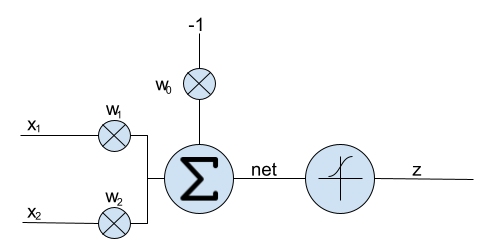
\includegraphics[width=0.6\linewidth]{../common/01_neuronal_network/00_resources/00_perceptron.png}
    \end{center}
    \caption{Das Perceptron}
    \label{fig:04_perceptron}
\end{figure}

Am Ende dieses Perceptrons steht die Berechnung eines Fehlers. An dieser Stelle wird die quadratische Distanz gewählt.
Man berechnet also die quadratische Differenz zwischen dem erwarteten Wert $d$ sowie dem effektiven Wert $z$.
\begin{align}
    P_{err} = \sum_i^n(d_i - z_i)^2
\end{align}
Im Falle des Perceptrons gibt es nur einen Output-Wert. Daher lässt sich die Fehlerfunktion wie in Gleichung \ref{eq:01_fehlerfunktion_perceptron}
darstellen.
\begin{align}
    P_{err} = (d - z)^2\label{eq:01_fehlerfunktion_perceptron}
\end{align}

\subsection{Lernverfahren}
Um nun die Gewichte entsprechend ihrem Anteil am Fehler zu korrigieren, wird das Gradientenabstiegsverfahren\footnote{Siehe Kapitel \ref{chapter:01_gradientenabstiegsverfahren}}
verwendet. Dazu muss die Ableitung der Fehlerfunktion bekannt sein. Um diese Ableitung einfacher zu gestalten,
wird die Fehlerfunktion mit einem konstanten Faktor $\frac{1}{2}$ multipliziert. Dieser Faktor hat keinen Einfluss
auf Minima oder Maxima, da er an jedem Punkt der Funktion angewendet wird.
\begin{align}
    P_{err} = \frac{1}{2} \cdot (d - z)^2
\end{align}
Nun hat eine Maximierung ebenfalls einen vereinfachenden Vorteil aufgrund der Kettenregel bei der Ableitungsbildung,
weswegen die Fehlerfunktion gedreht wird. Es ergibt sich die endgültige Fehlerfunktion.
\begin{align}
    P_{err} = -\frac{1}{2} \cdot (d - z)^2
\end{align}
Entsprechend lautet die Ableitung unter Anwendung der Kettenregel:
\begin{align}
    \frac{\delta P_{err}}{\delta z} = - \frac{1}{2} \cdot 2 \cdot (d - z) \cdot -1\\
    \frac{\delta P_{err}}{\delta z} = (d - z)
\end{align}

Die Gewichte können anhand des Gradienten korrigiert werden.
\begin{align}
    \begin{pmatrix}w_{0, neu} & w_{1, neu} & w_{2, neu}\end{pmatrix} = \begin{pmatrix}w_{0, alt} & w_{1, alt} & w_{2, alt}\end{pmatrix} + \lambda \cdot \vec{\nabla}
\end{align}
Dieser Gradient setzt sich aus der partiellen Ableitungskette der verschiedenen Funktionen nach den einzelnen
Gewichten zusammen, welche nacheinander aufgerufen werden und jeweils als Input für die Nächste dienen.
Dazu wird das Perceptron aus Abbildung \ref{fig:04_perceptron} von hinten her aufgerollt. Der Gradient lautet demnach:
\begin{align}
    \vec{\nabla} = \begin{pmatrix}\frac{\delta P_{err}}{\delta w_0} & \frac{\delta P_{err}}{\delta w_1} & \frac{\delta P_{err}}{\delta w_2} \end{pmatrix}
\end{align}
An dieser Stelle wird nun die Ableitungskette für $w_0$ näher erläutert. In einem ersten Schritt muss also die
Ableitung der Fehlerfunktion nach $w_0$ gebildet werden. Wie bereits erwähnt, werden die Funktionen nacheinander
aufgerufen und dienen sich gegenseitig als Input. Von hinten her aufgerollt lautet die Aufrufreihenfolge:
\begin{align}
    P_{err} = (d - z(net(w_0, w_1, w_2)))
\end{align}
Für $z$ und $net$ gilt:
\begin{align}
    z = \frac{1}{1 + e^{-net}}\\
    net = -1 \cdot w_0 + x_1 \cdot w_1 + x_2 \cdot w_2
\end{align}

Um den Wert des Gradienten für $w_0$ zu bilden, muss die Funktion $P_{err}$ für $w_0$ partiell abgeleitet
werden. Dies geschieht durch konsequentes Anwenden der Kettenregel.
\begin{align}
    \frac{\delta P_{err}}{\delta z(w_0)} = (d - z)\\
    \frac{\delta z(w_0)}{\delta net(w_0)} = z (1 - z)\\
    \frac{\delta net(w_0)}{\delta w_0} = -1
\end{align}

Die gesamte Ableitungskette nach Anwendung der Kettenregel lautet:
\begin{align}
    \frac{\delta P_{err}}{\delta w_0} = \frac{\delta P_{err}}{\delta z(w_0)} \cdot \frac{\delta z(w_0)}{\delta net(w_0)} \cdot \frac{\delta net(w_0)}{\delta w_0}\\
    \frac{\delta P_{err}}{\delta w_0} = (d - z) \cdot z \cdot (1 - z) \cdot -1\label{eq:02_ableitungskette_perceptron}
\end{align}
Mit dem Ausdruck \ref{eq:02_ableitungskette_perceptron} lässt sich das Gewicht $w_0$ in einer Iteration korrigieren.
Dasselbe Verfahren wird für die Gewichte $w_1$ sowie $w_2$ angewendet, es resultiert:
\begin{align}
    \frac{\delta P_{err}}{\delta w_1} = (d - z) \cdot z \cdot (1 - z) \cdot x_1\\
    \frac{\delta P_{err}}{\delta w_2} = (d - z) \cdot z \cdot (1 - z) \cdot x_2
\end{align}

\newpage
\subsection{Das Problem mit XOR und nichtlinearen Funktionen}\label{chapter:02_xor_perceptron}
Mittels eines Perceptrons kann also eine Funktion implementiert werden, die ab einer gewissen Schwelle den
Ausgabewert 1 liefert. Geometrisch kann dies als eine lineare Separation angesehen werden. Es können z.B. logische
Operatoren wie \glqq AND\grqq{}, \glqq OR\grqq{} oder auch \glqq NAND\grqq{} abgebildet werden.
In der Abbildung \ref{fig:06_logische_operatoren_1} werden die genannten Operatoren gezeigt. Auf den X-Y-Achsen
sind jeweils die Input-Variablen angegeben. Die Output-Dimension wird als Kreis dargestellt. Da der Input auf die Paare
$(x,y) \longrightarrow (0,0), (1,0), (0,1), (1,1)$ beschränkt ist, befinden sich die Output-Werte ebenfalls nur an diesen
Positionen. Wird an einer Stelle als Ausgabe eine $1$ erwartet, so ist der Kreis rot ausgefüllt. Wird eine $0$ erwartet,
ist der Kreis nicht ausgefüllt.
\begin{figure}[h!]
    \begin{center}
        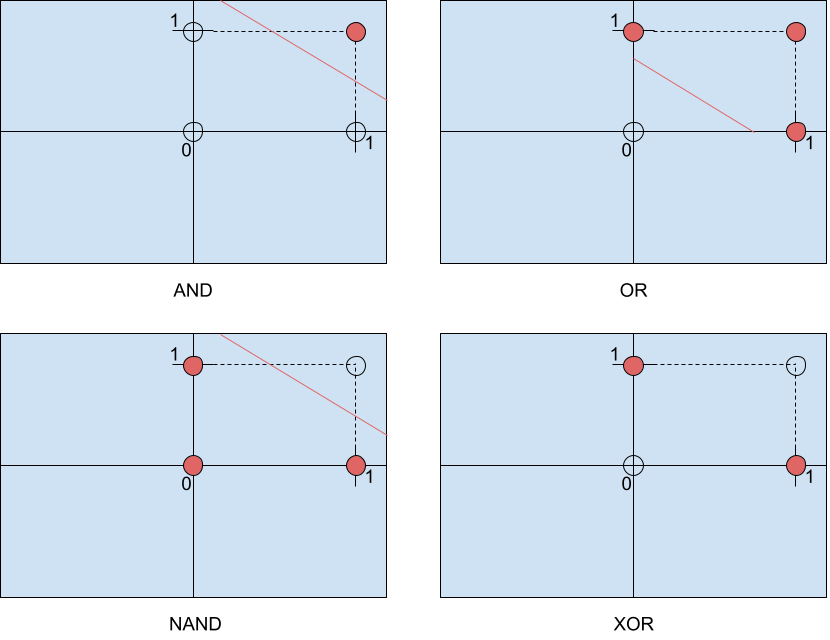
\includegraphics[width=0.6\linewidth]{../common/01_neuronal_network/00_resources/01_logische_operatoren.png}
    \end{center}
    \caption{Logische Operatoren und ihre Separierbarkeit}
    \label{fig:06_logische_operatoren_1}
\end{figure}
In Abbildung \ref{fig:06_logische_operatoren_1} wird gezeigt, was mit einem Perceptron möglich ist. Es können nur
Funktionen implementiert werden, die die einzelnen Klassen voneinander linear separieren können (durch die eingezeichnete
rote Gerade). Dies ist im Falle von \glqq XOR\grqq{} nicht möglich. Der Leser kann sich selbst überlegen, wie eine solche
Gerade auszusehen vermag, um eine Grenze zu ziehen. Diese Problematik soll durch ein neuronales Netz gelöst werden, wo
viele dieser Perceptronen miteinander verbunden sind. Dadurch ergeben sich weitere Möglichkeiten, um die Werte in
bestimmten Clustern zu klassifizieren. Es können also auch nichtlineare Funktionen abgebildet werden.